\documentclass[presentation]{beamer}
\usepackage{pgfgantt}
\usepackage[absolute,overlay]{textpos}
\usepackage{tikz}
\usetikzlibrary{calc,intersections}
\newsavebox\myAnim

\usepackage{pgfplots}
\pgfplotsset{plot coordinates/math parser=false}


\providecommand{\ro}[1]{\mathbf{r}_o}
\providecommand{\so}[1]{\mathbf{\hat{s}}_o}
\providecommand{\rb}[1]{\mathbf{r}_b}

\usepackage{animate}
\usepackage[utf8]{inputenc}
\usepackage[T1]{fontenc}
\usepackage{fixltx2e}
\usepackage{graphicx}
\usepackage{longtable}
\usepackage{float}
\usepackage{wrapfig}
\usepackage{rotating}
\usepackage[normalem]{ulem}
\usepackage{amsmath}
\usepackage{textcomp}
\usepackage{marvosym}
\usepackage{wasysym}
\usepackage{amssymb}
\usepackage{hyperref}
\usepackage{setspace}
\tolerance=1000
\usepackage{graphicx} \DeclareMathOperator{\argmin}{argmin}
\linespread{1}

\newcommand{\me}{\mathrm{e}}
\providecommand{\e}[1]{\ensuremath{\times 10^{#1}}} 
\providecommand{\mb}[1]{\mathbf{#1}}
\providecommand{\mf}[1]{\mathfrak{#1}}
\providecommand{\ro}[1]{\mathbf{\mathfrak{r}}_o}
\providecommand{\so}[1]{\mathbf{\hat{s}}_o}
\providecommand{\rb}[1]{\mathbf{r}_b}
\providecommand{\rbm}[1]{r_b^{\text{m}}}
\providecommand{\rd}[1]{\mathbf{r}_d}
\providecommand{\mh}[1]{\mathbf{\hat{#1}}}
\providecommand{\bs}[1]{\boldsymbol{#1}} 
\providecommand{\intinf}{\int_{-\infty}^{\infty}}
\newcommand{\under}[2]{\underset{\scriptscriptstyle#1}{#2}}

\usetheme{simple} \usecolortheme{} \usefonttheme{serif} \useinnertheme{}
\useoutertheme{}

\begin{document}
\begin{frame}{
    \vspace{0em}
    \begin{center}
      Live-Cell Biology with Three-Dimensional\\
      Fluorescence Orientation Microscopy
    \end{center}}
  \vspace{-2em}
  \centering
  \animategraphics[loop, autoplay, palindrome, width=0.65\linewidth, controls, buttonsize=0.5em]{10}{figs/recon/}{1}{164}
  \begin{center}
    \vspace{0em}
    Talon Chandler\\ \vspace{0.5em}
  March 21, 2018
  \end{center}
\end{frame}

\begin{frame}
  \begin{columns}[totalwidth=6cm]
    \begin{column}{.5\textwidth}
      \centering
      \onslide<1->{\textbf{PET/SPECT}}\\ \vspace{0.2em}
      \onslide<1->{\centering 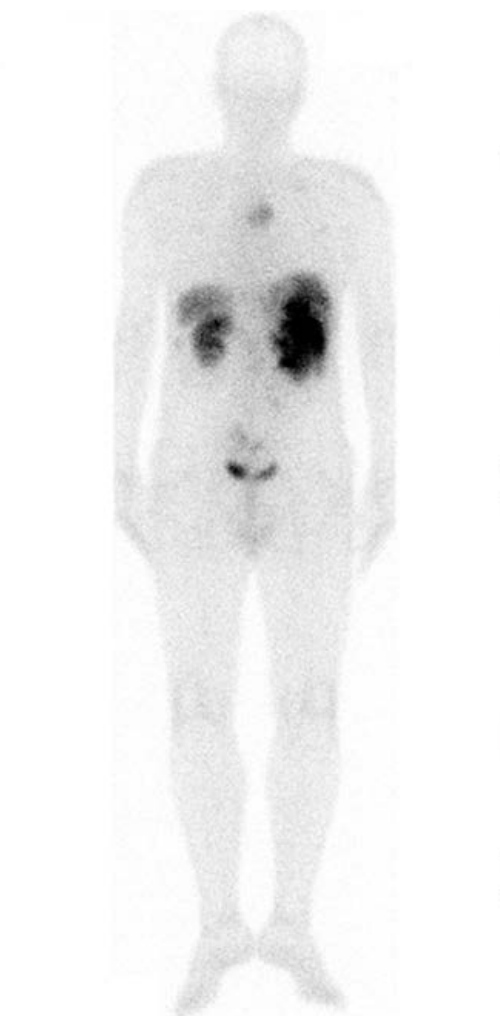
\includegraphics[width=0.35\textwidth]{figs/spect.png}}\\
      % Wong, 2017      
      \onslide<1->{Radionuclide}\\
      \onslide<1->{Human scale}\\
      \onslide<1->{Medical discovery}\\
      \vphantom{Orientation}
    \end{column}
    \begin{column}{.5\textwidth}
      \centering
      \onslide<2->{\textbf{Fluorescence Microscopy}}\\ \vspace{0.2em}
      \onslide<2->{\centering 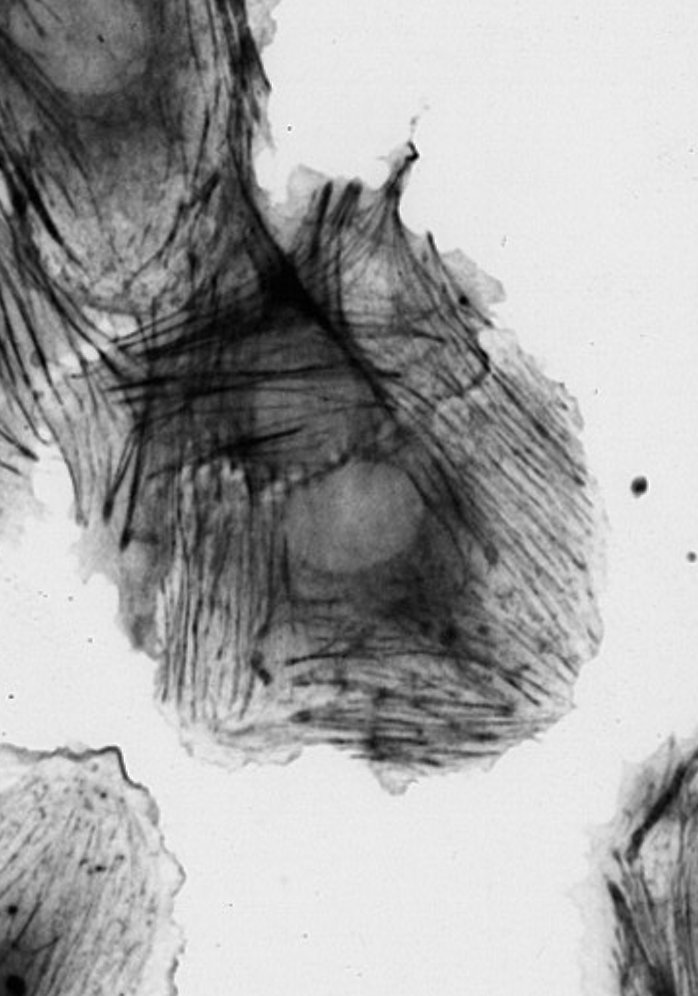
\includegraphics[width=0.52\textwidth]{figs/cellinv.jpg}}\\
      %Iacoviello, 1995
      \onslide<2->{Fluorophore}\\
      \onslide<2->{Cell scale}\\
      \onslide<2->{Biological discovery}\\
      \onslide<3->{Orientation}\\
    \end{column}
  \end{columns}
\end{frame}

\begin{frame}{Overview}
  % Position\\ \vspace{2em}
  % Orientation\\ \vspace{2em}
  % Proposal
\centering
\Large
\begin{tikzpicture}
  [thin/.style={text width=2.5cm, align=center}]
  \node (one) at (0,0) {Position};
  \node (two) [below=of one] {Orientation};
  \node (three) [below=of two] {Proposal};
  \node [thin] (a1) [below left=of three] {Aim 1:\\ Reconstruct};
  \node [thin] (a2) [below=of three] {Aim 2:\\ Verify};
  \node [thin] (a3) [below right=of three] {Aim 3:\\ Apply};    

  \draw [] (one.south) -- (two.north);
  \draw [] (two.south) -- (three.north);
  \draw [] (three.south west) -- (a1.north);
  \draw [] (three.south) -- (a2.north);
  \draw [] (three.south east) -- (a3.north);  
\end{tikzpicture}
  
\end{frame}

\begin{frame}[label=sec-1]{Part 1: Position}
 \begin{center}
   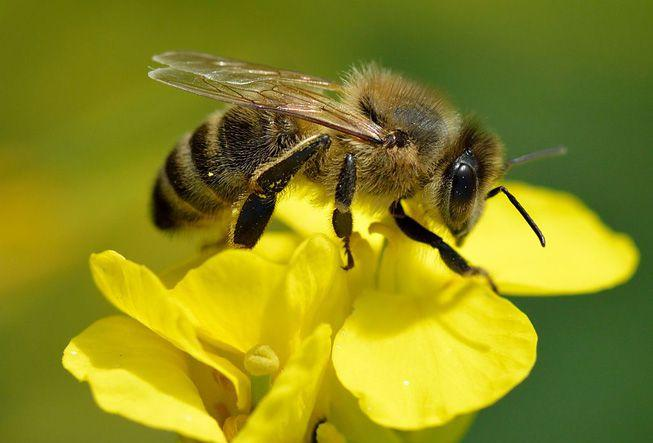
\includegraphics[width=0.8\textwidth]{figs/bee1.jpg}
%http://mediad.publicbroadcasting.net/p/wnmu/files/styles/x_large/public/201712/bee.jpg
 \end{center}
\end{frame}

\begin{frame}{Fluorescence microscope}
  \centering
    \animategraphics[loop, width=0.9\textwidth]{10}{figs/microscope/microscope}{0}{29}  
\end{frame}  

\begin{frame}{Where can we find fluorescent samples?} 
  \begin{columns}
    \begin{column}{.33\textwidth}
      \centering
      \onslide<1->{Endogenous}\\ \vspace{0.2em}
      \onslide<1->{\centering 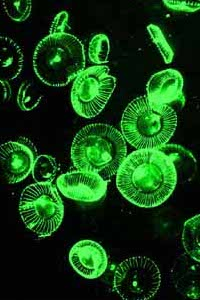
\includegraphics[width=1.0\textwidth]{figs/aequoria.jpg}}\\
      %http://lem.ch.unito.it/didattica/infochimica/2008_GFP/estrazione.html
    \end{column}
    \begin{column}{.33\textwidth}
      \centering
      \onslide<3->{Genetic}\\ \vspace{0.2em}
      \onslide<3->{\centering 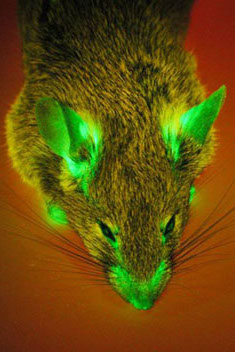
\includegraphics[width=1.0\textwidth]{figs/GFP_mouse.jpg}}\\
      %http://sites.udel.edu/art-in-science/2016/02/18/green-fluorescent-protein-illuminating-molecular-level-processes/
    \end{column}
    \begin{column}{.33\textwidth}
      \centering
      \onslide<2->{Exogeneous}\\ \vspace{0.2em}
      \onslide<2->{\centering 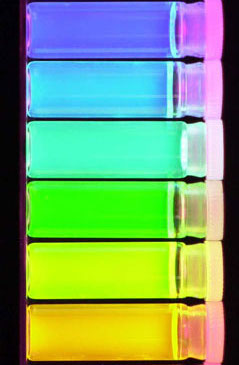
\includegraphics[width=1.0\textwidth]{figs/dyes.jpg}}\\
      % http://www.healthfreedoms.org/fluorescent-dyes-light-up-brain-cancer-cells/
    \end{column}
  \end{columns}
\end{frame}

\begin{frame}[label=sec-1]{What can we study?}
  \begin{center}
    \includegraphics[width=0.8\textwidth]{figs/yeast/yeast-gfp.png}
    \vphantom{\raisebox{-10pt}{\makebox[0pt][r]{\footnotesize DeMay, 2011}}}
\end{center}
\setlength{\TPHorizModule}{\textwidth}
 \setlength{\TPVertModule}{\textwidth}
\begin{textblock}{0.5}(0.1,0.26)
  \rotatebox[origin=c]{90}{DIC}
 \end{textblock}
\end{frame}

\begin{frame}[label=sec-1]{What can we study?}
  \begin{center}
    \includegraphics[width=0.8\textwidth]{figs/yeast/yeast-gfp-all.png}
    \raisebox{-10pt}{\makebox[0pt][r]{\footnotesize DeMay, 2011}}
\end{center}
\setlength{\TPHorizModule}{\textwidth}
\setlength{\TPVertModule}{\textwidth}
\begin{textblock}{0.5}(0.1,0.26)
  \rotatebox[origin=c]{90}{DIC}
 \end{textblock}
\begin{textblock}{0.49}(0.1,0.48)
  \rotatebox[origin=c]{90}{Fluorescence}
 \end{textblock}

\end{frame}

\begin{frame}{Review}
  \centering
  \Large
  Biological question\\ $\downarrow$ \\
  Fluorescent labeling\\ $\downarrow$ \\
  Microscopic imaging \\ $\downarrow$ \\
  Biological conclusion
\end{frame}

\begin{frame}[label=sec-1]{Part 2: Orientation}
 \begin{center}
   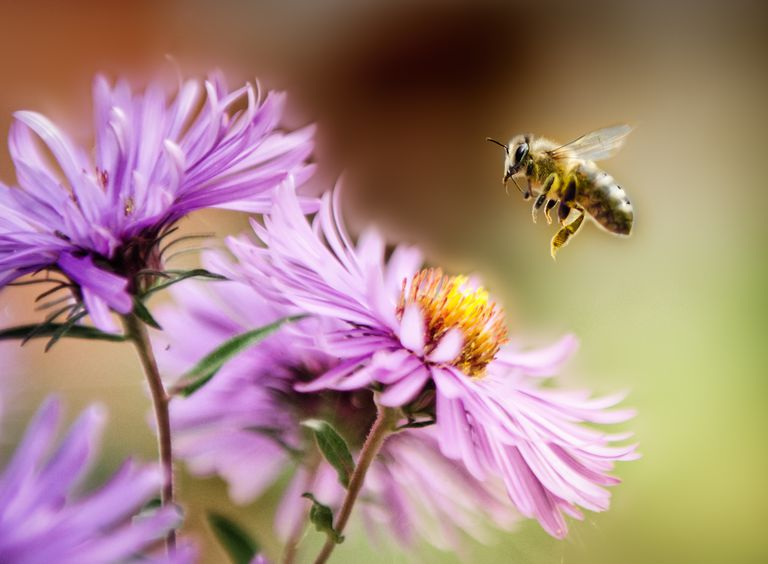
\includegraphics[width=0.8\textwidth]{figs/bee2.jpg}
%https://www.thoughtco.com/how-to-save-the-worlds-bees-1140836
 \end{center}
\end{frame}

\begin{frame}{Fluorescence microscope}
  \centering
    \animategraphics[loop, width=0.9\textwidth]{10}{figs/microscope/microscope}{0}{29}  
\end{frame}  
\begin{frame}{\centering Monopole $\neq$ Dipole}
  \vspace{1em}
  \begin{columns}
    \begin{column}{.5\textwidth}
      \centering Monopole emitter \\ \vspace{.5em}
    \animategraphics[loop, width=0.9\textwidth]{10}{figs/monopole/monopole}{}{}
  \end{column}
  \begin{column}{.5\textwidth}
    \centering Dipole emitter \\ \vspace{.5em}
    \animategraphics[loop, width=0.9\textwidth]{10}{figs/dipole/dipole}{}{}
  \end{column}    
\end{columns}
\centering
\vspace{0.5em}
\pause
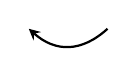
\begin{tikzpicture}
  \draw[->, thick, -stealth] (0,0) .. controls (-0.33,-0.3) and (-0.66,-0.3) .. (-1,0);
\end{tikzpicture}\\ \vspace{0.25em}
quickly rotating dipoles\\
or\\
many dipoles in all orientations \\
\end{frame}  

\begin{frame}{Polarized light}
  \begin{center}
        \animategraphics[loop, width=0.7\textwidth]{10}{figs/xpol/xpol}{0}{29}   \end{center}
\end{frame}

\begin{frame}{Polarized light}
  \begin{center}
        \animategraphics[loop, width=0.7\textwidth]{10}{figs/ypol/ypol}{0}{29}   \end{center}
    \end{frame}

\begin{frame}{Monopole $\neq$ Dipole}
  \vspace{3em}
  \begin{columns}
    \begin{column}{.5\textwidth}
      \centering Monopole absorber \\ \vspace{.5em}
      \animategraphics[loop, width=0.9\textwidth]{10}{figs/monopole-excite/monopole}{}{}
      \vspace{-3em}\\ All fields\\ excite a monopole. 
  \end{column}
  \begin{column}{.5\textwidth}
    \centering Dipole absorber \\ \vspace{.5em}
    \animategraphics[loop, width=0.9\textwidth]{10}{figs/dipole-excite/dipole}{}{}
    \vspace{-3em}\\ Parallel component of the fields\\ excite a dipole. 
  \end{column}    
\end{columns}
\centering
\vspace{0.5em}
\end{frame}

\begin{frame}{Two ways to measure the dipole axis}
  \centering
  \Large
  Polarized excitation\\ \vspace{1em}
  Polarized detection
\end{frame}

\begin{frame}{Microscopes can find fluorophores}
  \begin{center}
    \includegraphics[width=0.8\textwidth]{figs/yeast/yeast-gfp-all.png}
    \raisebox{-10pt}{\makebox[0pt][r]{\footnotesize DeMay, 2011}}
\end{center}
\setlength{\TPHorizModule}{\textwidth}
\setlength{\TPVertModule}{\textwidth}
\begin{textblock}{0.49}(0.1,0.26)
  \rotatebox[origin=c]{90}{DIC}
 \end{textblock}
\begin{textblock}{0.49}(0.1,0.48)
  \rotatebox[origin=c]{90}{Fluorescence}
\end{textblock}
\end{frame}

\begin{frame}{Single-view polarized fluorescence microscope}
  \begin{center}
    \begin{tikzpicture}
    \node[anchor=south west,inner sep=0] (image) at (0,0) {\includegraphics[scale=0.2]{figs/fluo-pol.pdf}};
    \node[anchor=south west,inner sep=0] (image) at (7.5,-1.67) {\includegraphics[scale=0.57]{figs/single-arm-schematic.png}};
    \draw[thin, dashed] (4.4,1.9) -- (9.3, 1.9);
  \end{tikzpicture}
  \end{center}
\end{frame}

\begin{frame}{Polarized light microscopes reveal molecular order}
 \begin{center}
   \includegraphics[width=0.8\textwidth]{figs/yeast/yeast-orientation.png}
   \raisebox{-10pt}{\makebox[0pt][r]{\footnotesize DeMay, 2011}}
 \end{center}
\end{frame}

\begin{frame}{Review}
  \centering
  \Large
  Biological question\\ $\downarrow$ \\
  \textbf{Orientational}\\ fluorescent labeling\\ $\downarrow$ \\
  \textbf{Orientational}\\ microscopic imaging \\ $\downarrow$ \\
  Biological conclusion
\end{frame}

\begin{frame}{Existing techniques}
   \begin{center}
     \includegraphics[width=0.8\textwidth]{figs/existing.png}\\
   \end{center}
   \tiny
   \vfill
   S. B. Mehta, M. McQuilken, P. J. La Rivi\`{e}re, P. Occhipinti, A. Verma, R.
   Oldenbourg, A. S. Gladfelter, and T. Tani, ``Dissection of molecular assembly
   dynamics by tracking orientation and position of single molecules in live
   cells,'' Proc. Natl. Acad. Sci. U.S.A. 113, E6352–E6361 (2016).\\
   \vspace{0.5em}
   A. Agrawal, S. Quirin, G. Grover, and R. Piestun, ``Limits of 3D dipole
   localization and orientation estimation for single-molecule imaging: towards
   Green’s tensor engineering,'' Opt. Express 20, 26667–26680 (2012).
\end{frame}

\begin{frame}[label=sec-1]{Part 3: Proposal}
 \begin{center}
   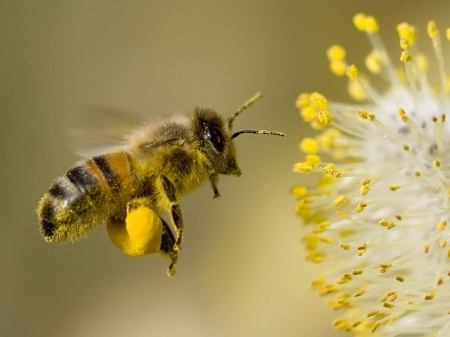
\includegraphics[width=0.8\textwidth]{figs/bee3.jpg}
%https://www.bee-america.com/content/5-things-about-bees-will-amaze-you
 \end{center}
\end{frame}

\begin{frame}{Proposal Summary}
  \begin{center}
  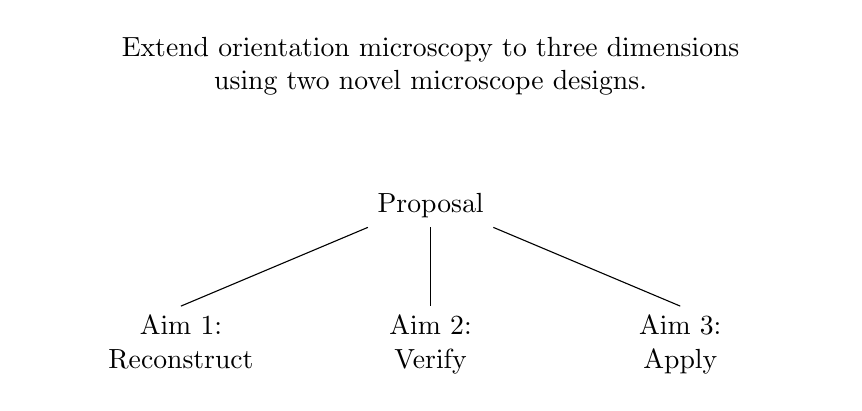
\begin{tikzpicture}
    [thick/.style={text width=10cm, align=center},
    thin/.style={text width=2.5cm, align=center}]    
  \node [thick] (two) {Extend orientation microscopy to three dimensions\\
    using two novel microscope designs.};
  \node (three) [below=of two] {Proposal};
  \node [thin] (a1) [below left=of three] {Aim 1:\\ Reconstruct};
  \node [thin] (a2) [below=of three] {Aim 2:\\ Verify};
  \node [thin] (a3) [below right=of three] {Aim 3:\\ Apply};    

  \draw [] (three.south west) -- (a1.north);
  \draw [] (three.south) -- (a2.north);
  \draw [] (three.south east) -- (a3.north);  
\end{tikzpicture}
\end{center}
\end{frame}

\begin{frame}[label=sec-1]{Dual-view microscope}
 \begin{center}
   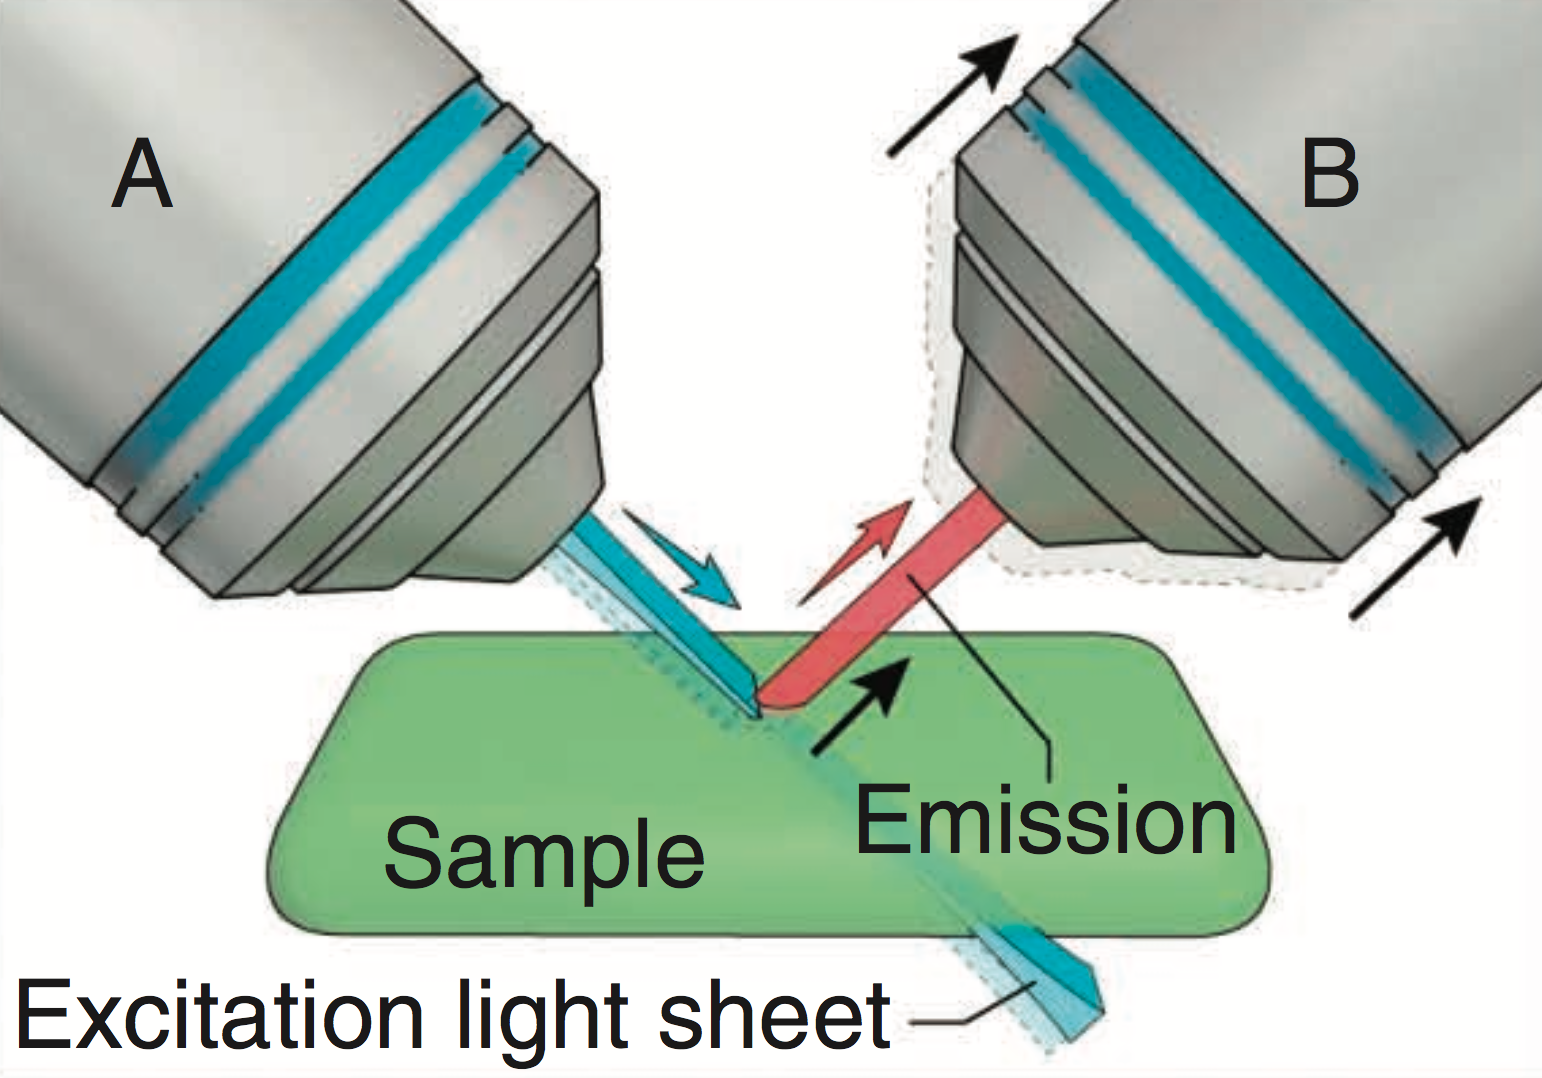
\includegraphics[width=0.7\textwidth]{figs/light-sheet.png}
   \raisebox{-10pt}{\makebox[0pt][r]{\footnotesize Wu, 2013}}
 \end{center}
\end{frame}

\begin{frame}[label=sec-1]{Orientation uncertainty study}
  \vspace{0.5em}
 \begin{center}
   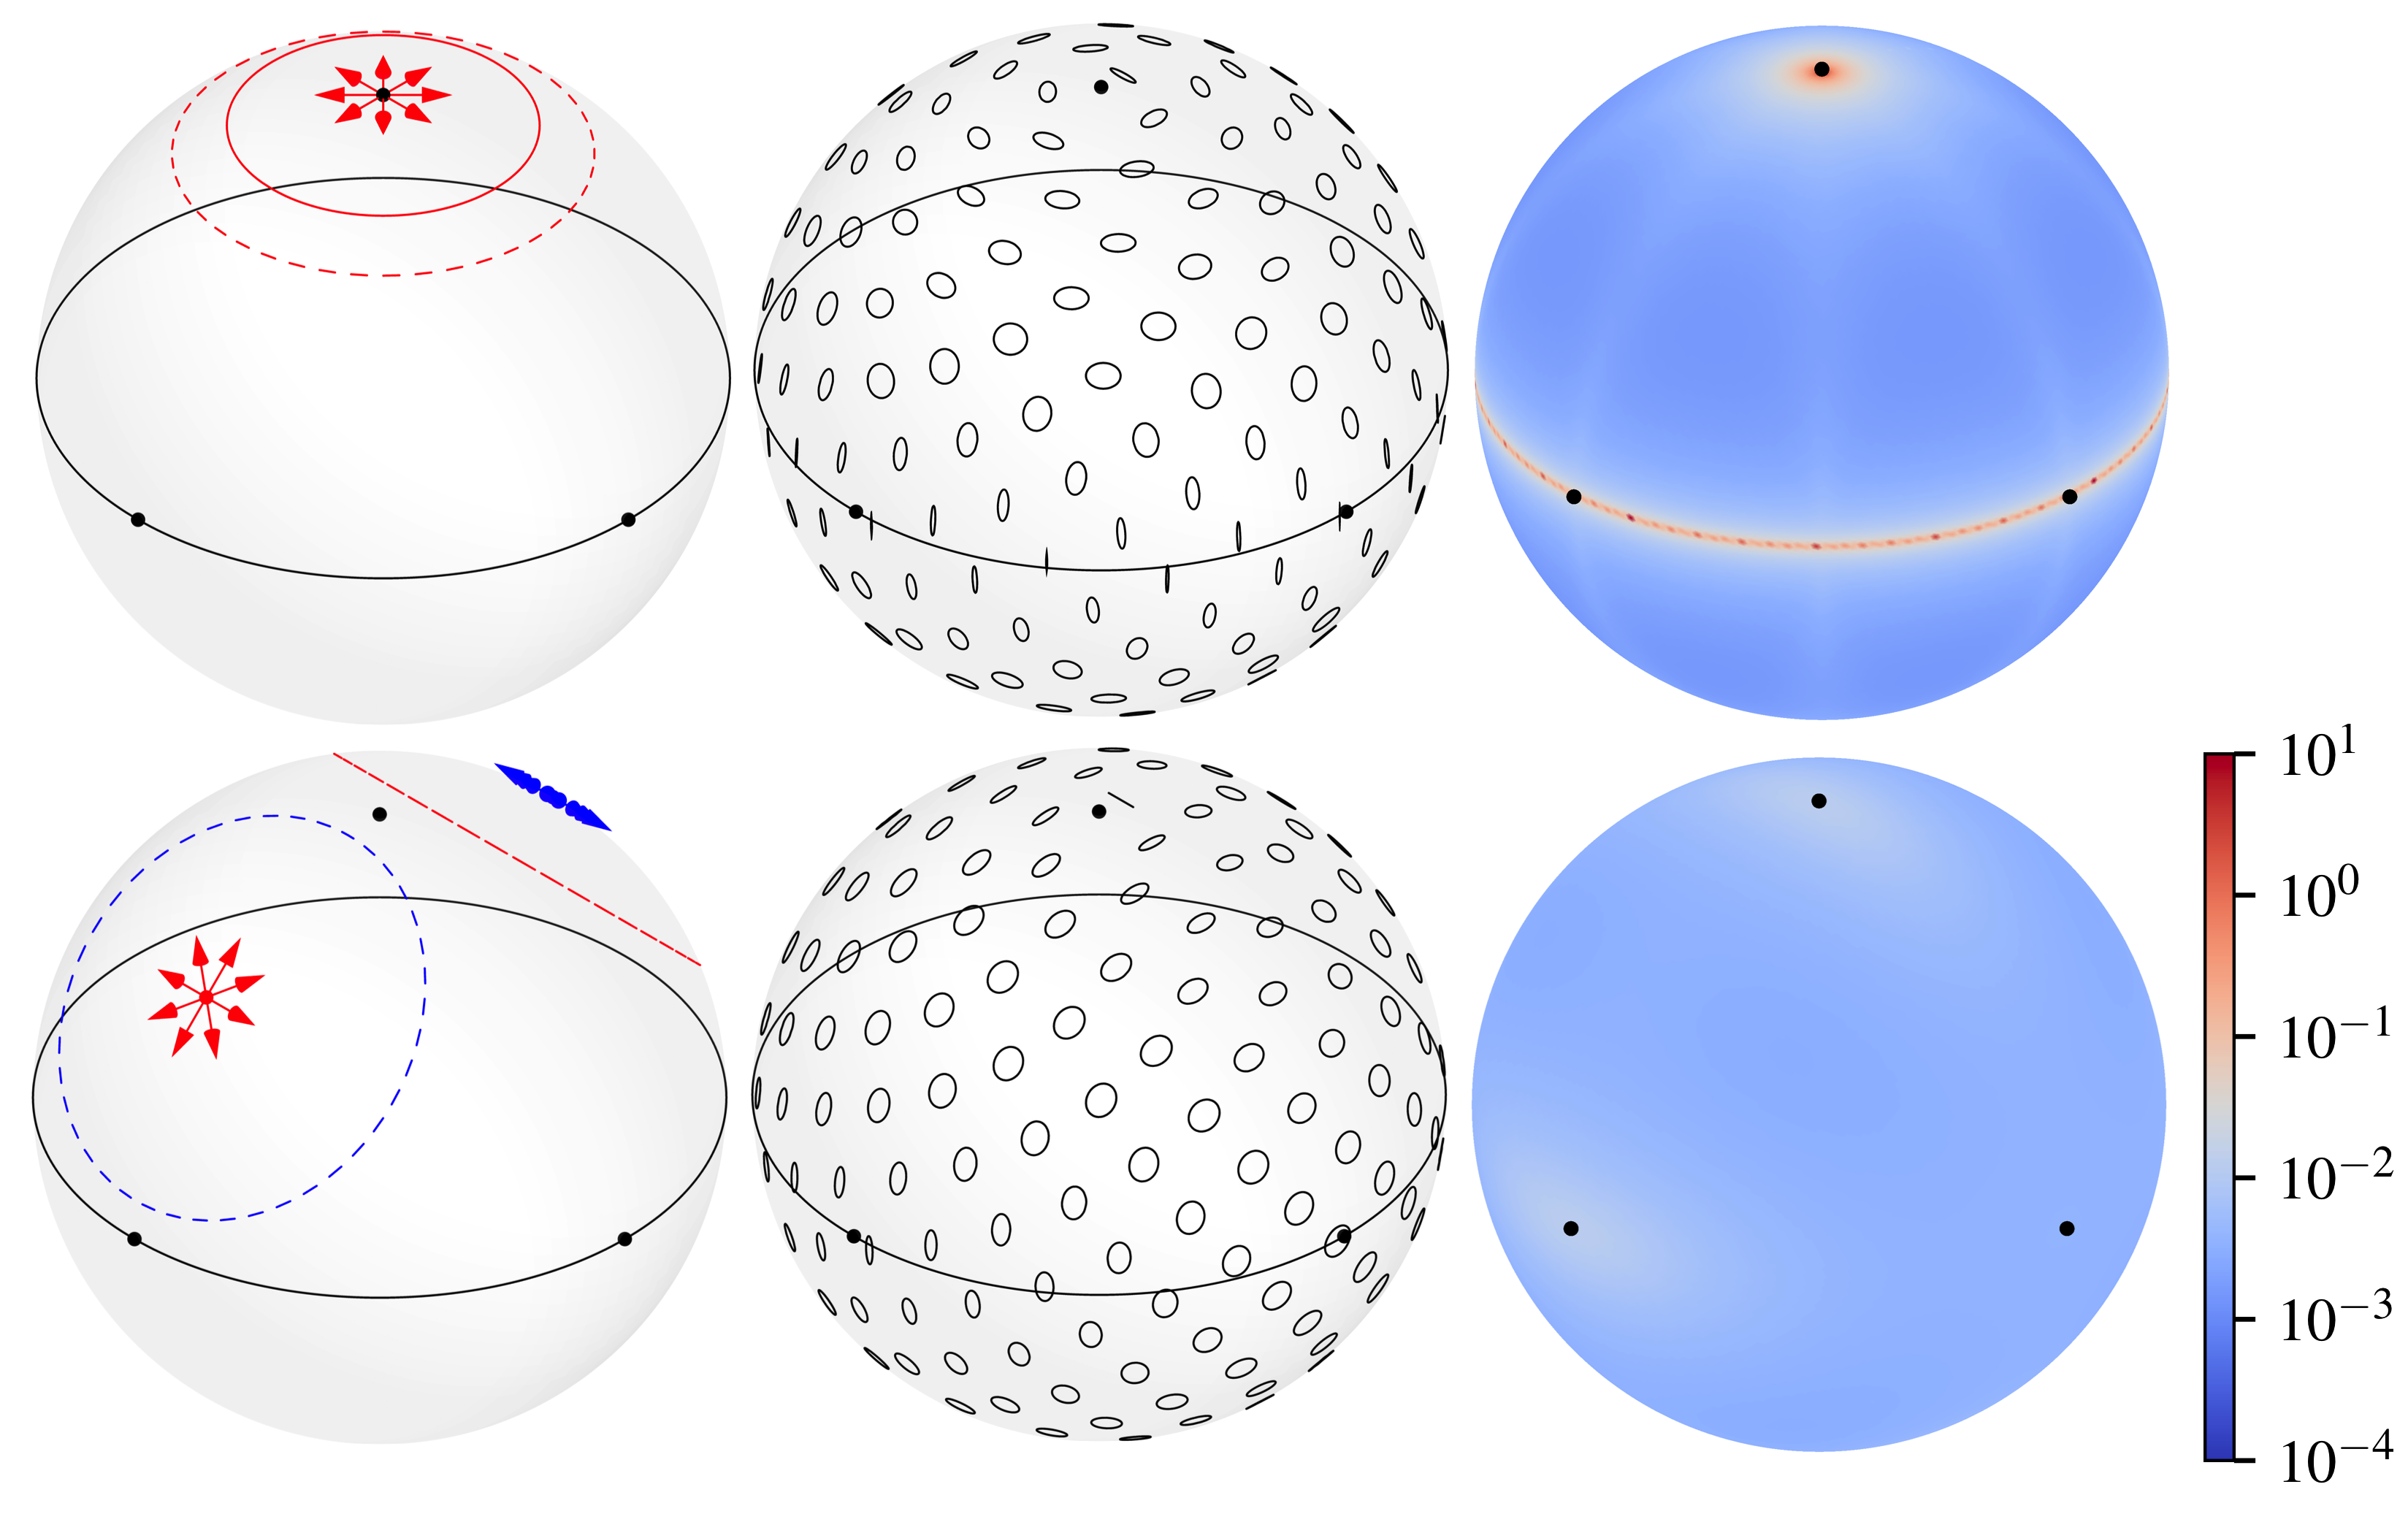
\includegraphics[width=0.75\textwidth]{figs/proposal-fig.png}
   \raisebox{-10pt}{\makebox[0pt][r]{\footnotesize Chandler, 2017}}
 \end{center}
 Dual-view microscopes can measure the orientation of single molecules with less
 uncertainty and fewer degeneracies.
 \small
 \setlength{\TPHorizModule}{\textwidth}
 \setlength{\TPVertModule}{\textwidth}
\begin{textblock}{0.5}(0.13,0.18)
  \rotatebox[origin=c]{90}{Single-view}
\end{textblock}
\begin{textblock}{0.5}(0.13,0.4)
  \rotatebox[origin=c]{90}{Dual-view}
\end{textblock}
\begin{textblock}{0.5}(0.04,0.1)
  \centering
  Geometry
 \end{textblock}
 \begin{textblock}{0.5}(0.25,0.08)
   \centering
  Relative\\ Uncertainty
\end{textblock}
\begin{textblock}{0.5}(0.48,0.08)
  \centering  
  Absolute\\ Uncertainty [sr]
\end{textblock}
\end{frame}


\begin{frame}[label=sec-1]{Lightfield microscope}
 \begin{center}
   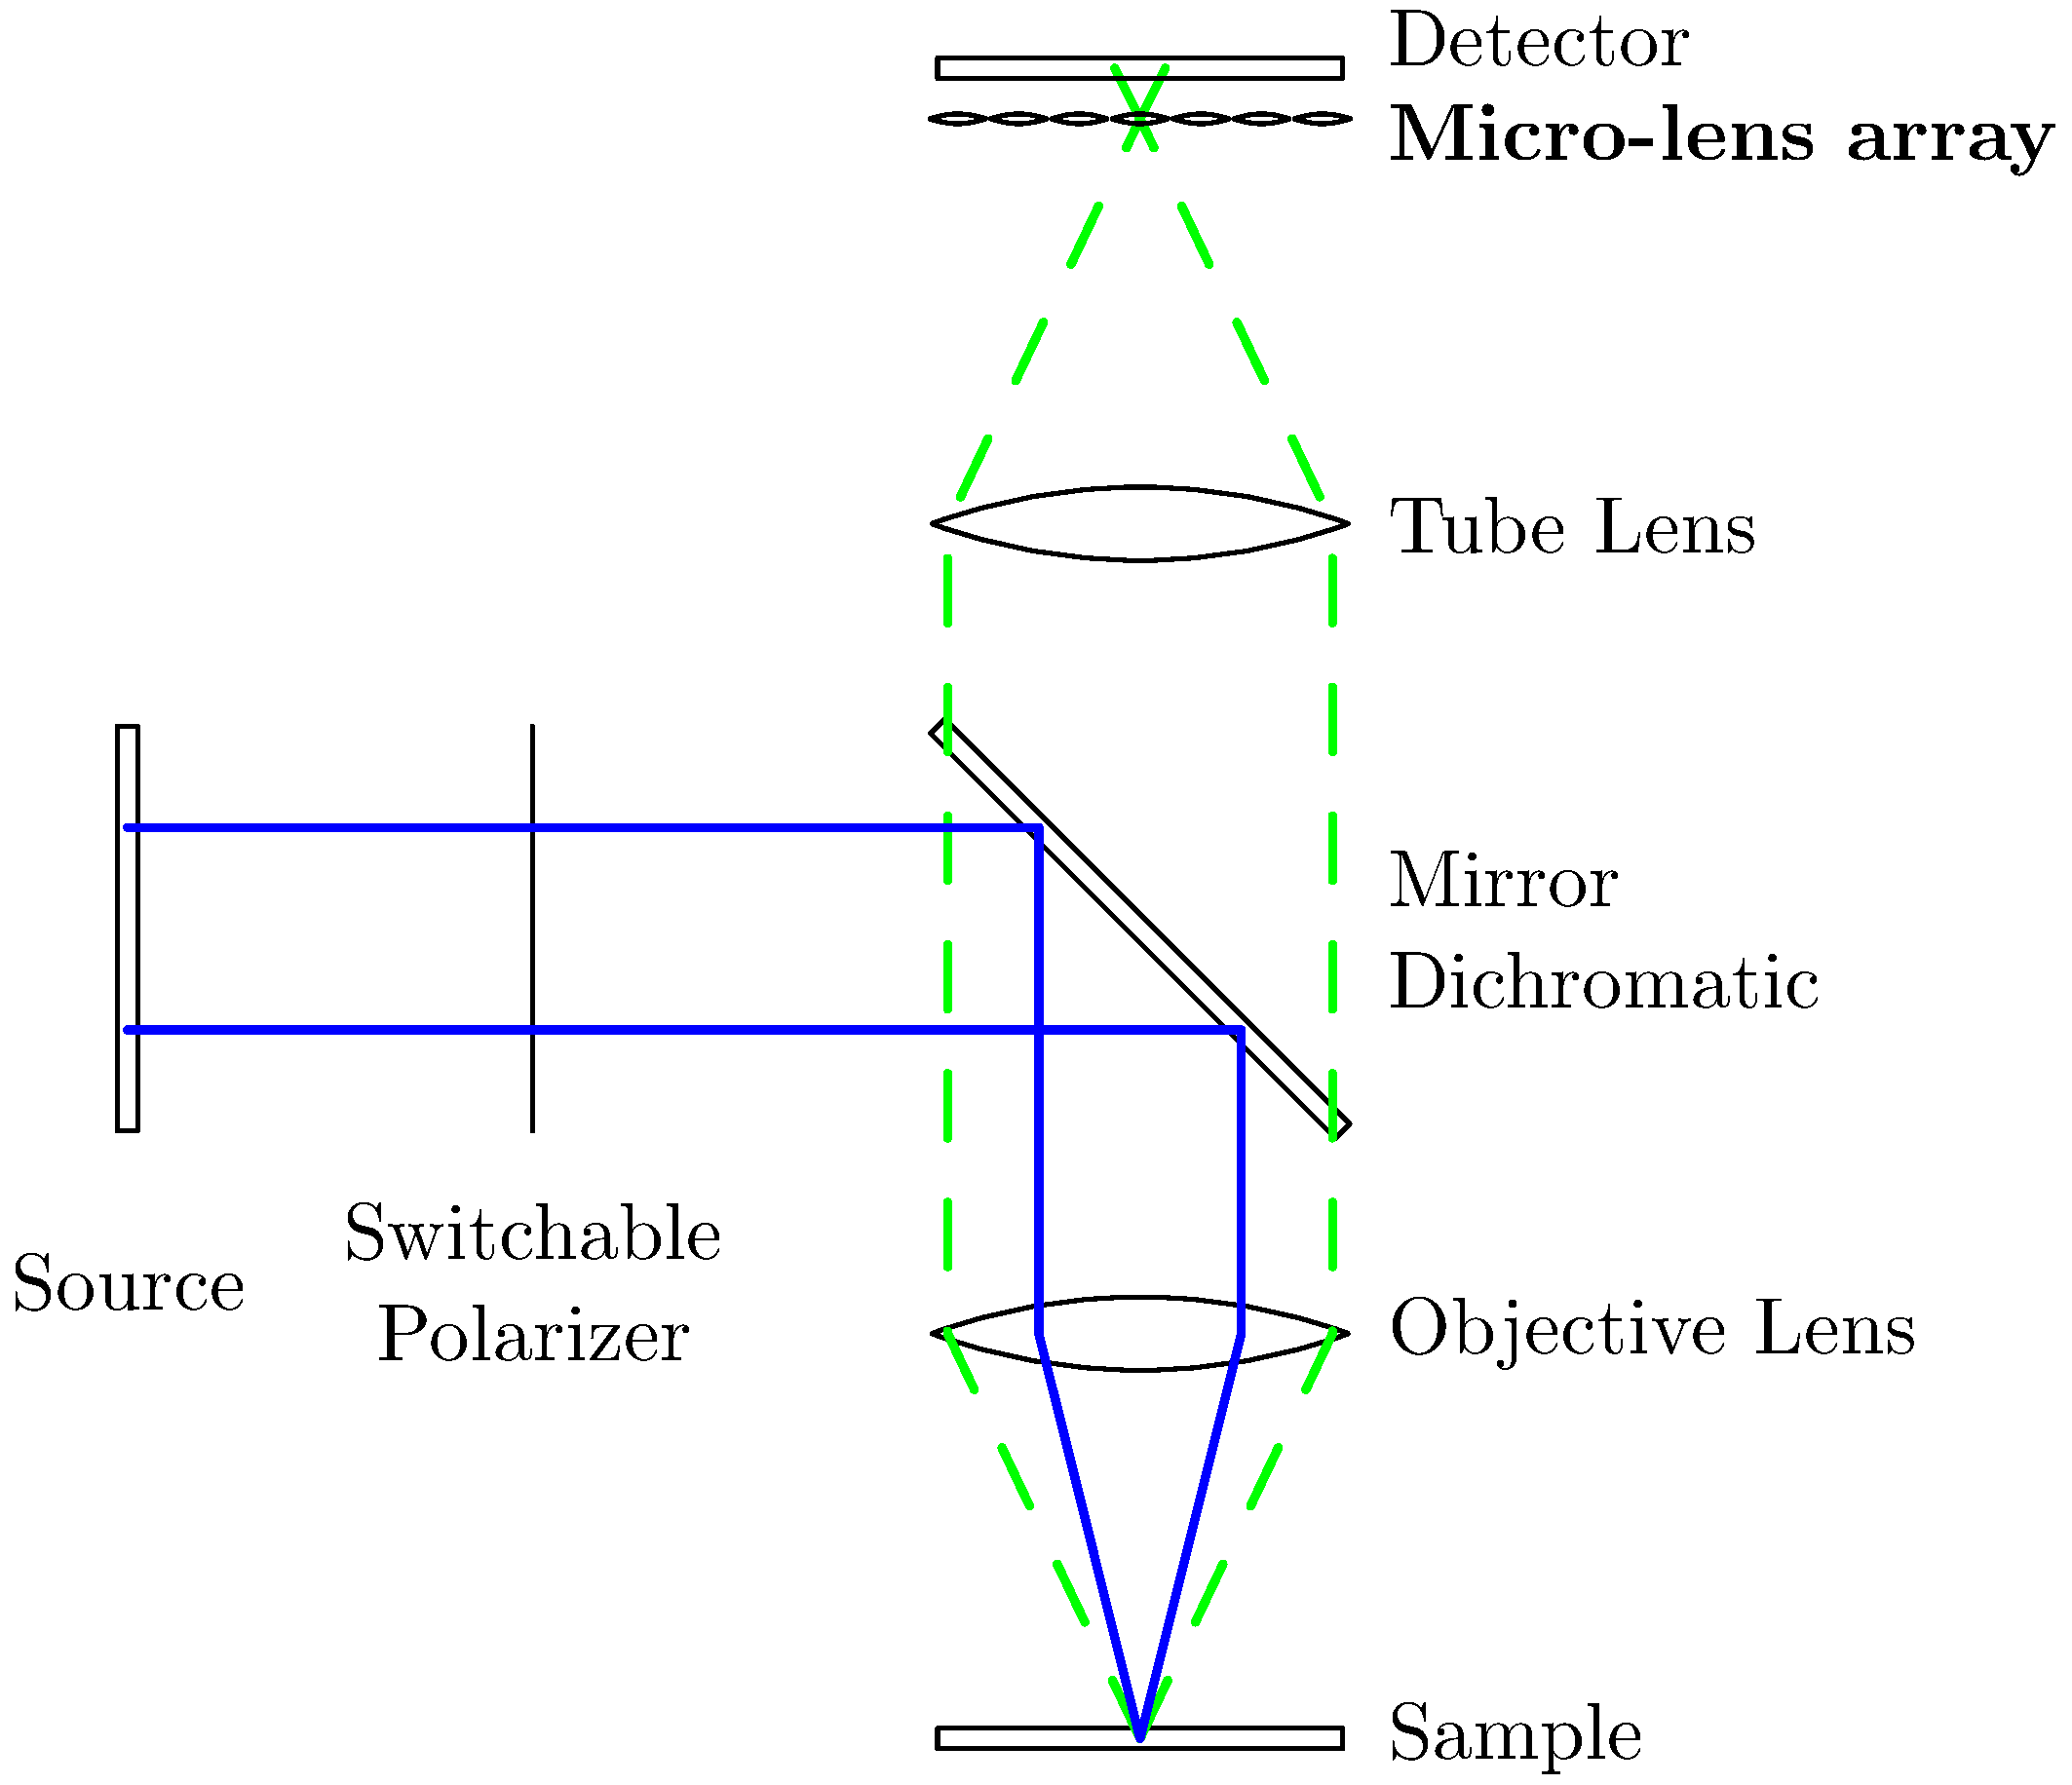
\includegraphics[width=0.7\textwidth]{figs/fluo-lf.pdf}
 \end{center}
\end{frame}

\begin{frame}[label=sec-1]{Lightfield microscope}
 \begin{center}
   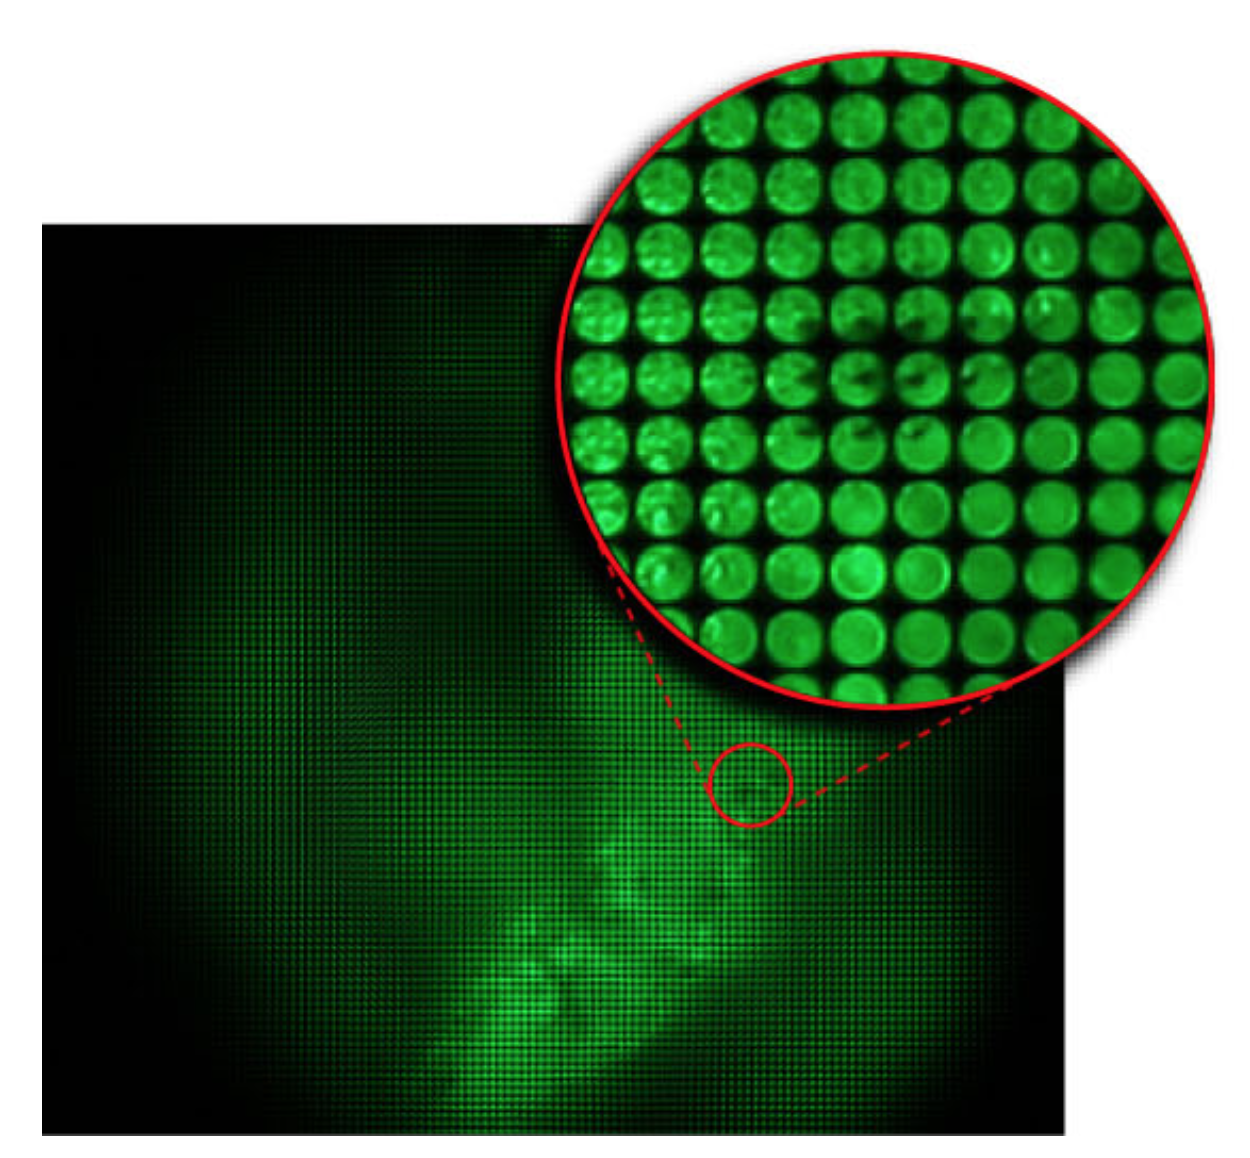
\includegraphics[width=0.7\textwidth]{figs/levoy/lf-fluo.png}
   \raisebox{-10pt}{\makebox[0pt][r]{\footnotesize Levoy, 2006}}
 \end{center}
\end{frame}

\begin{frame}[label=sec-1]{Lightfield microscope}
 \begin{center}
   \includegraphics[width=1.0\textwidth]{figs/levoy/refocus.png}
   \raisebox{-10pt}{\makebox[0pt][r]{\footnotesize Levoy, 2006}}
 \end{center}
\end{frame}

\begin{frame}{Proposed techniques}
   \begin{center}
     \includegraphics[width=0.9\textwidth]{figs/proposed.png}\\ \vspace{1.5em}
     Major bottleneck: reconstruction schemes.
   \end{center}
   
\end{frame}


\begin{frame}{}
  \begin{center}
    \textbf{Aim 1:}\\ \vspace{1em}
    Develop a three-dimensional orientation reconstruction pipeline.
  \end{center}
\end{frame}

\begin{frame}{Forward model}
  \begin{align*}
    \underbrace{\vphantom{\int_{\mathbb{R}^3}}g_i(\rd{})}_{\substack{\text{Detected} \\ \text{intensities}}}
    =
    \underbrace{\int_{\mathbb{R}^3}d\ro{} \int_{\mathbb{S}^2}d\so{}}_{\substack{\text{Integral over position} \\ \text{and orientation}}}
    \underbrace{\vphantom{\int_{\mathbb{R}^3}}h_i(\rd{}; \ro{}, \so{})}_{\substack{\text{Spatio-angular}\\ \text{point spread function}}}
    \underbrace{\vphantom{\int_{\mathbb{R}^3}}f(\ro{}, \so{})}_{\substack{\text{Spatio-angular}\\ \text{density}}}
  \end{align*}
  \begin{center}
    \vspace{1em}
    \small{$i$ indexes polarizations or views}
  \end{center}
\end{frame}

\begin{frame}[label=sec-1]{Spatial harmonics}
 \begin{center}
   \includegraphics[width=0.8\textwidth]{figs/harmonics/harmonics.pdf}
 \end{center}
\end{frame}

\begin{frame}[label=sec-1]{Spherical harmonics}
 \begin{center}
   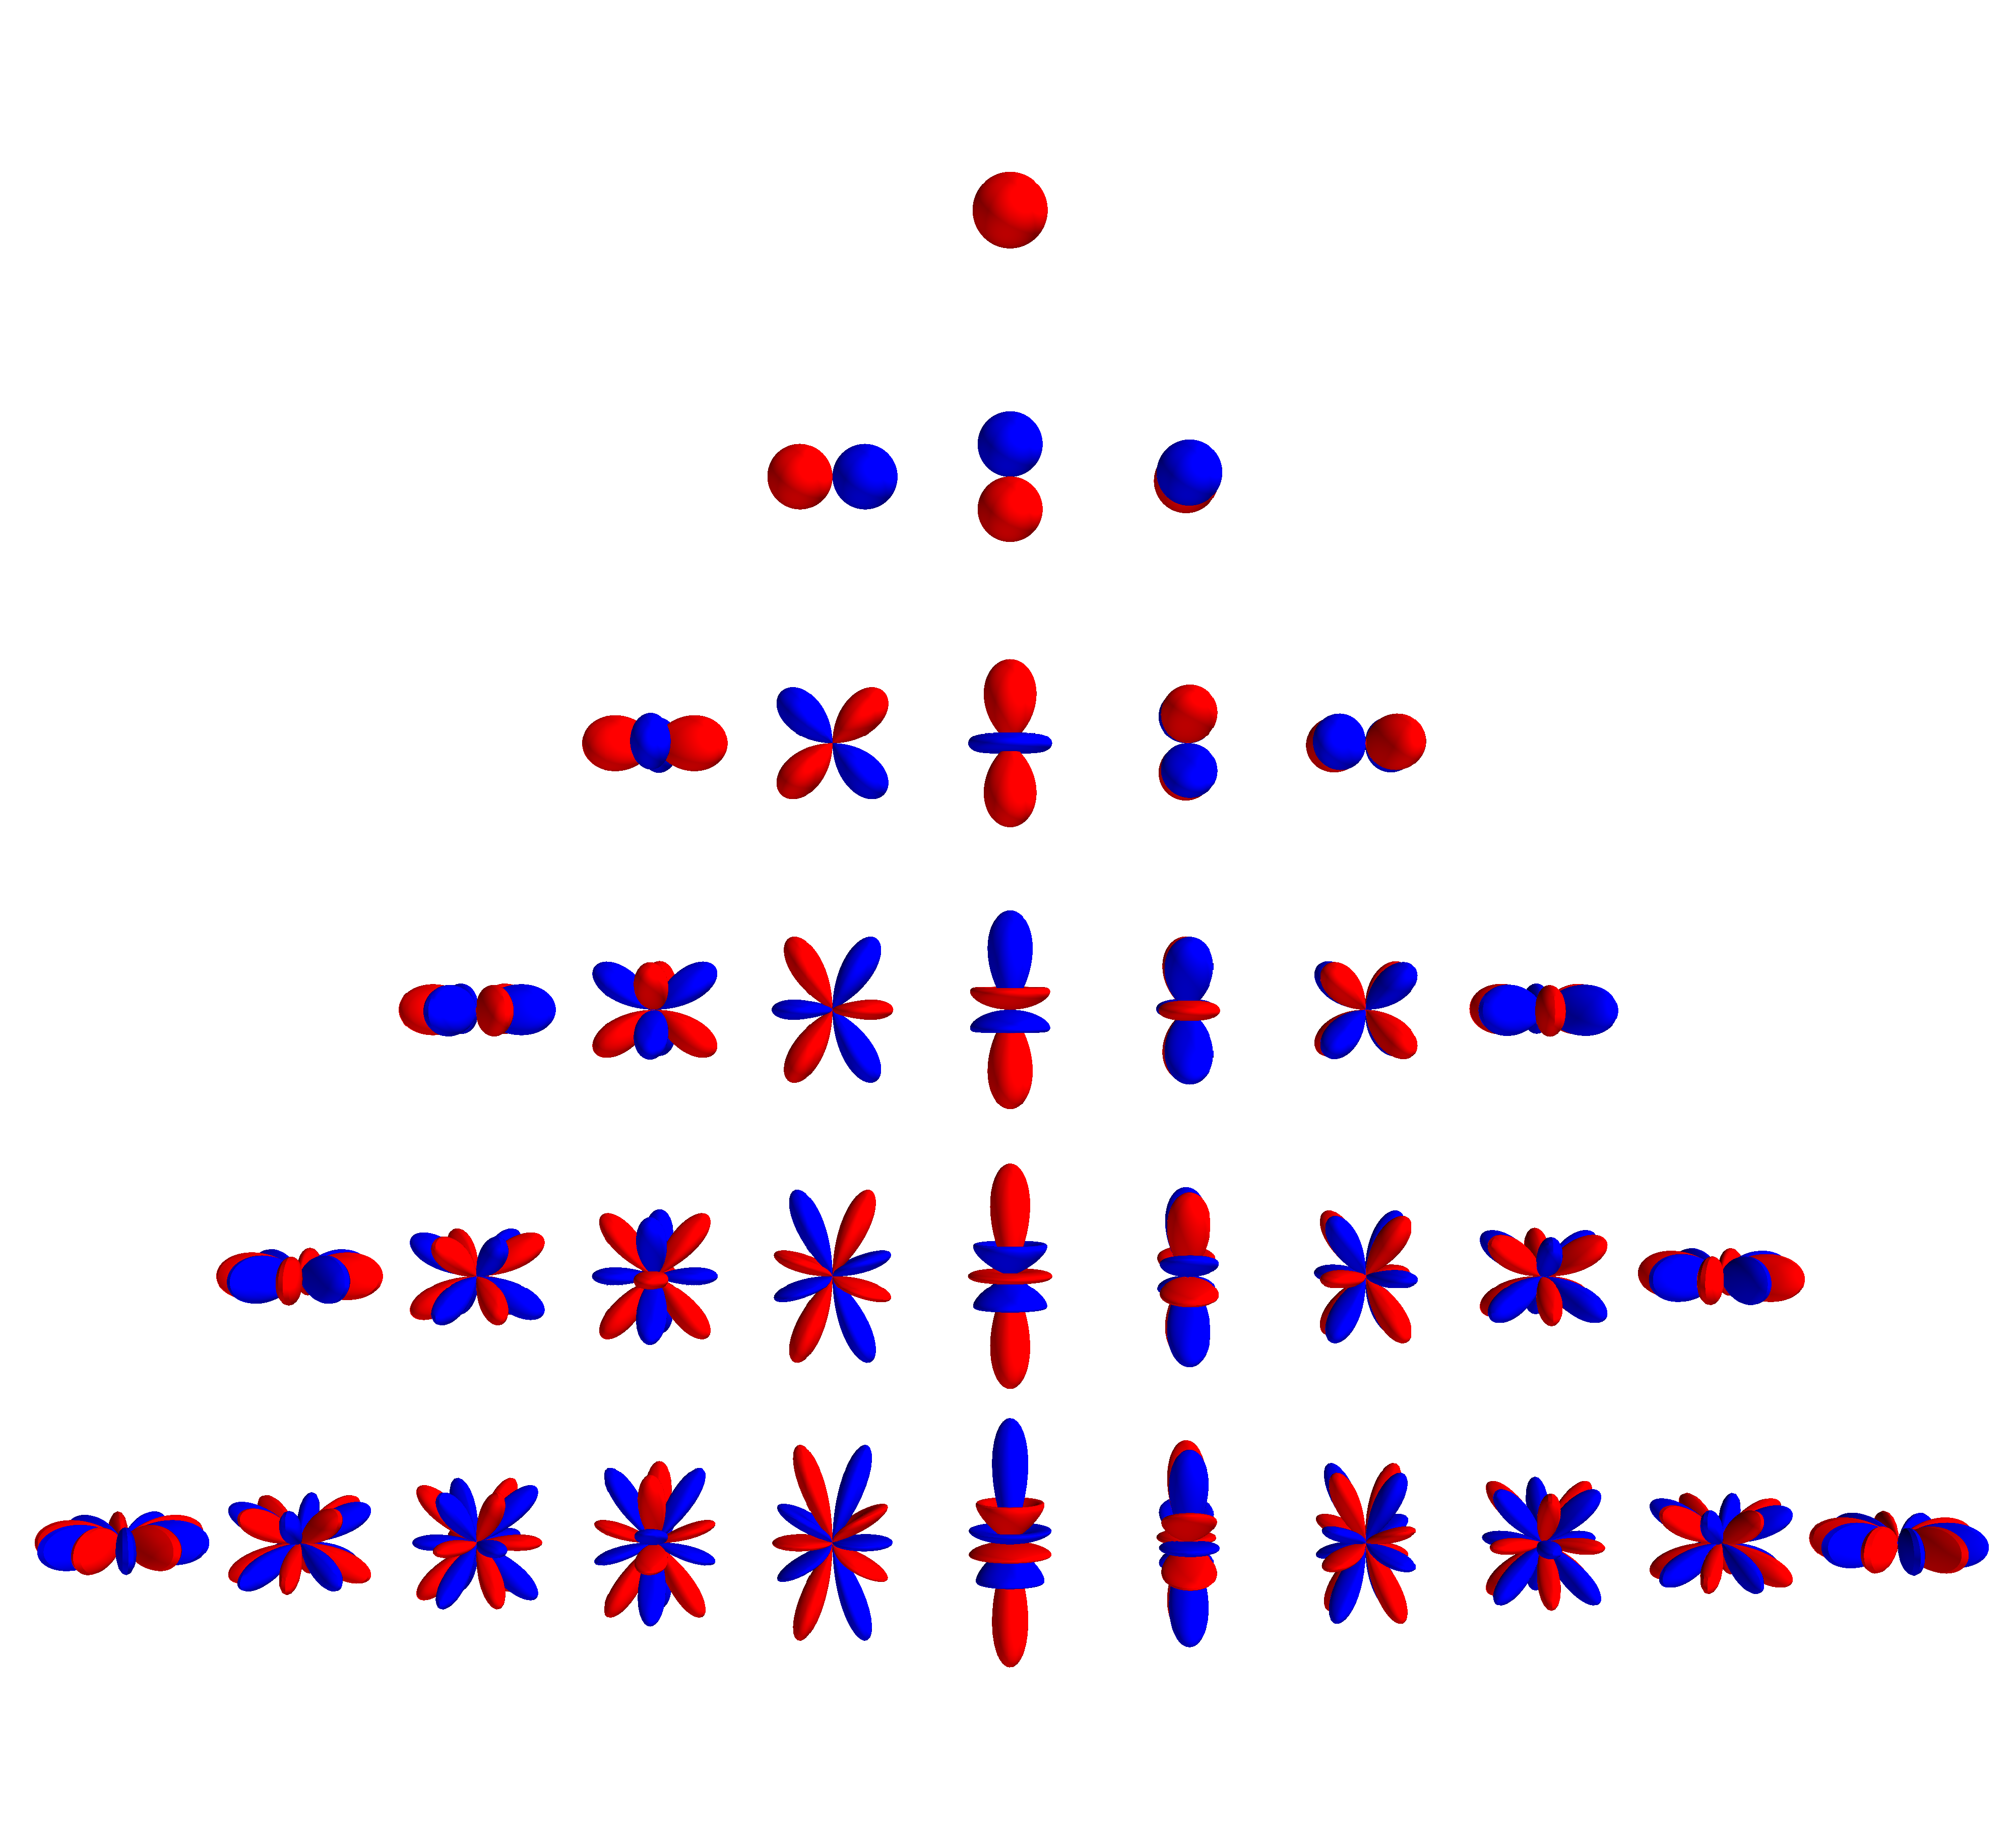
\includegraphics[width=0.8\textwidth]{figs/sph_harm.png}
 \end{center}
\end{frame}

\begin{frame}{Forward model}
  \begin{align*}
    \underbrace{\vphantom{\int_{\mathbb{R}^3}}g_i(\rd{})}_{\substack{\text{Detected} \\ \text{intensities}}}
    =
    \underbrace{\int_{\mathbb{R}^3}d\ro{} \int_{\mathbb{S}^2}d\so{}}_{\substack{\text{Integral over position} \\ \text{and orientation}}}
    \underbrace{\vphantom{\int_{\mathbb{R}^3}}h_i(\rd{}; \ro{}, \so{})}_{\substack{\text{Spatio-angular}\\ \text{point spread function}}}
    \underbrace{\vphantom{\int_{\mathbb{R}^3}}f(\ro{}, \so{})}_{\substack{\text{Spatio-angular}\\ \text{density}}}
  \end{align*}
  \begin{center}
    \vspace{1em}
    \small{$i$ indexes polarizations or views}
  \end{center}
  
  \begin{itemize}
  \item Spherical harmonic expansion: \begin{align*}f(\ro{}, \so{}) = \sum_{l=0}^{\infty}\sum_{m=-l}^{l}F_l^m(\ro{})y_l^m(\so{}) \end{align*}
  \item Shift invariant: $h_i(\rd{}; \ro{}, \so{}) \rightarrow h_i(\rd{} - \ro{}, \so{})$
  \item Separable: $h_i(\rd{}; \ro{}, \so{}) \rightarrow h_i^1(\rd{}; \ro{})h_i^2(\so{})$
  \end{itemize}
\end{frame}

\begin{frame}[label=sec-1]{Dual-view angular singular value spectrum}
 \begin{center}
   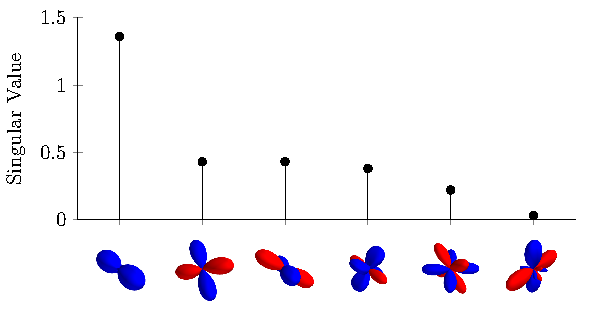
\includegraphics[width=0.8\textwidth]{figs/svs_dispim.pdf}
 \end{center}
\end{frame}

\begin{frame}[label=sec-1]{Reconstructions}
  \begin{align*}
\mathbf{f^{\thinspace *}}= \underset{\mathbf{f}}{\text{argmin}}
\ \ ||\thinspace\mathbf{g} - \mathbf{H}\mathbf{f}\thinspace||_2^2
  \end{align*} \vspace{1.5em}
  \centering 
  \begin{itemize}
  \item Investigate least-squares and MLEM solutions---\\alternatives if necessary.
  \item Regularize for specific cases---Tikhonov, total variation, sparsity.
  \end{itemize}

\end{frame}

\begin{frame}[label=sec-1]{Asymmetric dual-view microscope data}
  \vspace{1.5em}
 \begin{center}
   \includegraphics[width=0.75\textwidth]{figs/MP/mp-assembled.pdf}
 \end{center}
 \setlength{\TPHorizModule}{\textwidth}
 \setlength{\TPVertModule}{\textwidth}
\begin{textblock}{0.5}(0.13,0.4)
  \rotatebox[origin=c]{90}{View}
\end{textblock}
\begin{textblock}{0.5}(0.47,0.1)
  {Polarizer setting}
 \end{textblock}

\end{frame}

\begin{frame}{Asymmetric dual-view microscope reconstruction}
  \centering
  \animategraphics[loop, controls, palindrome, autoplay, width=0.9\linewidth,
  buttonsize=0.5em]{10}{figs/recon/}{1}{164}
\end{frame}

\begin{frame}[label=sec-1]{Group theory for finding degeneracy}
\begin{columns}
  \begin{column}{0.5\textwidth}
    \centering \textbf{Quantum mechanics}\\\vspace{2em}
    $\mathcal{H} = \text{Hamiltonian}$\\\vspace{2em}
    $\mathcal{H}\psi_k = W_k\psi_k$\\\vspace{2em}
    $\mathcal{T}_j\mathcal{H} - \mathcal{H}\mathcal{T}_j = 0$\\\vspace{2em}
    $\mathcal{T}_j$ form the symmetry group of the Hamiltonian.
\end{column}
\begin{column}{0.5\textwidth}  %%<--- here
  \centering \textbf{Imaging science}\\\vspace{2em}
  $\mathcal{H} = \text{Forward operator}$\vspace{2em}
  $\mathcal{H}^{\dagger}\mathcal{H}u_k = \mu_ku_k$\\\vspace{2em}
  $\mathcal{T}_j\mathcal{H}^{\dagger}\mathcal{H} - \mathcal{H}^{\dagger}\mathcal{H}\mathcal{T}_j = 0$\\\vspace{2em}
  $\mathcal{T}_j$ form the symmetry group of the imaging system.
  \end{column}
\end{columns}
\end{frame}

\begin{frame}{Aim 1 Summary}
  \begin{columns}
    \begin{column}{0.75\textwidth}
    Develop a three-dimensional orientation reconstruction pipeline.\\ \vspace{1em}
    \textbf{Subaim 1:} 
    Develop a complete signal processing theory for orientation microscopes. \\ \vspace{1em}
    \textbf{Subaim 2:}
    Implement reconstruction algorithms for dual-view and lightfield microscopes.\\ \vspace{1em}
    \textbf{Subaim 3:}
    Develop a visualization tool for interpreting 6D reconstructions. 
    \end{column}
  \end{columns}
  \end{frame}

\begin{frame}{}
  \begin{center}
    \textbf{Aim 2:}\\ \vspace{1em}
    Verify three-dimensional orientation microscopy.
  \end{center}
\end{frame}

\begin{frame}{Known coupling between position and orientation}
  \begin{columns}
    \begin{column}{0.5\textwidth}
       \begin{center}
   \includegraphics[width=0.8\textwidth]{figs/guv.jpg}\\ \vspace{0.5em}
    Giant unilamellar vesicles
  \end{center}
    \end{column}
    \begin{column}{0.5\textwidth}
       \begin{center}
   \includegraphics[width=0.8\textwidth]{figs/actin3.jpg}\\ \vspace{0.5em}
    Actin networks
  \end{center}
    \end{column}
  \end{columns}
\end{frame}

\begin{frame}{Aim 2 Summary}
  \begin{columns}
    \begin{column}{0.75\textwidth}
    Verify three-dimensional orientation microscopy.\\ \vspace{1em}
    \textbf{Subaim 1:} 
    Find or make suitable spatio-angular phantoms. \\ \vspace{1em}
    \textbf{Subaim 2:}
    Image these phantoms with dual-view and lightsheet microscopes.\\ \vspace{1em}
    \textbf{Subaim 3:}
    Verify that reconstructions match expectations within $\sim 5^{\circ}$ and $\sim 200$ nm. 
    \end{column}
  \end{columns}
  \end{frame}

\begin{frame}{}
  \begin{center}
    \textbf{Aim 3:}\\ \vspace{1em}
    Demonstrate the value of three-dimensional
    orientation microscopy\\ for live-cell biology.
  \end{center}
\end{frame}

\begin{frame}{View biological processes in six dimensions}
  \begin{center}
    \includegraphics[width=0.5\textwidth]{figs/yeast/yeast-orientation.png}\\
    \includegraphics[width=0.7\textwidth]{figs/yeast/septin3d.png}
   \raisebox{-10pt}{\makebox[0pt][r]{\footnotesize DeMay, 2011}}
 \end{center}
\end{frame}

\begin{frame}{Potential applications:}
  \begin{columns}
    \begin{column}{0.5\textwidth}
      \begin{center}
      \includegraphics[width=0.7\textwidth]{figs/yeast-bud.png}\\  
      \end{center}
      Cell growth and division---septin network dynamics in yeast with Dr.~Amy~Gladfelter. 
    \end{column}
    \begin{column}{0.5\textwidth}
      \begin{center}
      \includegraphics[width=0.7\textwidth]{figs/actin.png}\\  
      \end{center}
      Cell migration---actin network dynamics in model cells with Dr.~Clare~Waterman.
    \end{column}
\end{columns}
\end{frame}

\begin{frame}{Aim 3 Summary}
  \begin{columns}
    \begin{column}{0.75\textwidth}
    Demonstrate the value of three-dimensional
    orientation microscopy for live-cell biology.\\ \vspace{1em}
    \textbf{Subaim 1:} 
    Identify potential biological specimens. \\ \vspace{1em}
    \textbf{Subaim 2:}
    Image these specimens with dual-view and lightsheet microscopes.\\ \vspace{1em}
    \textbf{Subaim 3:}
    Carry out a hypothesis-driven study alongside a biologist.
    \end{column}
  \end{columns}
  \end{frame}

\begin{frame}{Specific aims}
  \begin{columns}
    \begin{column}{0.75\textwidth}
    Extend orientation microscopy to three dimensions
    using dual-view and light-field microscopy.\\ \vspace{1em}
    \textbf{Aim 1:} 
    Develop a reconstruction pipeline.\\ \vspace{1em}
      \textbf{Aim 2:}
    Verify with known samples.\\ \vspace{1em}
      \textbf{Aim 3:}
    Apply to live-cell biology.  
    \end{column}
  \end{columns}
\end{frame}

\begin{frame}{Timeline}
  \centering
  \includegraphics[width=0.95\linewidth]{./figs/timeline.png}
\end{frame}

\begin{frame}[label=sec-20]{Contributors}
\begin{columns}
\begin{column}{0.25\textwidth}
\centering  \vspace{-1em}
\begin{figure}[t]
\includegraphics[width=.9\linewidth]{./figs/collab/ro.jpg}
\end{figure}\vspace{-1em}
Rudolf\\ Oldenbourg
\begin{figure}[t]
\includegraphics[width=.9\linewidth]{./figs/collab/gh.jpg}
\end{figure}\vspace{-1em}
Grant\\ Harris
\end{column}
\begin{column}{0.25\textwidth}
\centering  \vspace{-1em}
\begin{figure}[t]
\includegraphics[width=.9\linewidth]{./figs/collab/sm.jpg}
\end{figure}\vspace{-1em}
Shalin\\ Mehta
\begin{figure}[t]
\includegraphics[width=.9\linewidth]{./figs/collab/hs.jpg}
\end{figure}\vspace{-1em}
Hari\\Shroff
\end{column}
\begin{column}{0.25\textwidth}
\centering  \vspace{-1em}
\begin{figure}[t]
\includegraphics[width=.9\linewidth]{./figs/collab/mt.jpg}
\end{figure}\vspace{-1em}
Mai\\ Tran
\begin{figure}[t]
\includegraphics[width=.9\linewidth]{./figs/collab/mg.jpg}
\end{figure}\vspace{-1em}
Min\\ Guo 
\end{column}
\begin{column}{0.25\textwidth}
\centering  \vspace{-1em}
\begin{figure}[t]
\includegraphics[width=.9\linewidth]{./figs/collab/av.jpg}
\end{figure}\vspace{-1em}
Amitabh\\ Verma
\begin{figure}[t]
\includegraphics[width=.9\linewidth]{./figs/collab/plr.jpg}
\end{figure}\vspace{-1em}
 Patrick\\ La Rivi\`ere
\end{column}
\end{columns}
\end{frame}

\begin{frame}{Bibliography}\small
\textbf{Published:}  \\ \vspace{0.5em}
\textbf{T. Chandler}, S. Mehta, H. Shroff, R. Oldenbourg, and P. La Rivière, ``Single-fluorophore orientation determination with multiview polarized illumination: modeling and microscope design,'' Opt. Express  25, 31309-31325 (2017).\\

\textbf{T. Chandler}, S. Mehta, H. Shroff, R. Oldenbourg, and P. La Rivière, ``Single-fluorophore orientation determination with multiview polarized illumination microscopy,'' IEEE International Symposium on Biomedical Imaging (ISBI) Conference, (2018).\\ \vspace{1em}

\textbf{In review:}\\ \vspace{0.5em}
\textbf{T. Chandler}, M. Guo, S. Mehta, A. Kumar, H. Shroff, R. Oldenbourg, and P. La Rivière, ``Three-dimensional fluorophore orientation imaging with multiview polarized microscopy,'' Optics Society of America (OSA) Mathematics in Imaging Conference, (2018).\\

\textbf{T. Chandler}, M. Guo, H. Shroff, R. Oldenbourg, P. La Rivière,
``Spatio-angular restoration of fluorescence microscopy data,'' Gordon Research
Conference on Image Science, (2018). \\
\end{frame}

\begin{frame}{Funding}
  \begin{columns}
    \begin{column}{0.75\textwidth}
      University of Chicago Biological Sciences\\ Division Graduate Fellowship \vspace{1em}\\
      NIH R01GM114274\\ \vspace{1em}
      NIH R01EB017293\\
    \end{column}
  \end{columns}
\end{frame}

\begin{frame}[label=sec-1]{\centering Thank you!}
 \begin{center}
   \includegraphics[width=0.8\textwidth]{figs/bee4.jpg}
 \end{center}
\end{frame}


\end{document}